\documentclass{standalone}

\usepackage[OT1]{fontenc}
\renewcommand*\familydefault{\sfdefault}
\usepackage{helvet,sfmath}
\usepackage{siunitx}

\usepackage{tikz}
\usetikzlibrary{arrows,calc,patterns}
\usepackage{tikz,tkz-euclide}

\usetikzlibrary{decorations.markings}

%% midarrow
\tikzset{
    mid arrow/.style={
        decoration={markings, mark=at position 0.5 with {\arrow{stealth}}},
        postaction={decorate}
    }
}

%% Color
\definecolor{Wave}{RGB}{3, 49, 161}  % #0331A1
\definecolor{M_dipole}{RGB}{0, 127, 189} % #007FBD
\definecolor{J_Current}{RGB}{91, 199, 225} % #5BC7E1
\definecolor{Orange_note}{RGB}{248, 136, 16} % #F88810
\definecolor{P_dipole}{RGB}{201, 1, 161}  % #C901A1
\definecolor{E}{RGB}{113, 11, 121} % #710B79

\begin{document}

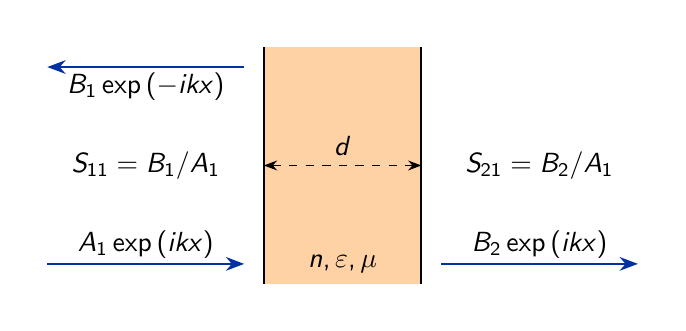
\begin{tikzpicture}[scale=0.5]
    %% Background
    \draw[draw=none] (-8,-3.5) rectangle (8,3.5);

    %% Material
    \draw[draw=none, fill=orange!35] (-2,-3) rectangle (2,3);
    \draw[thick]
    (-2,-3) to (-2,3)
    (2,-3) to (2,3)
    ;

    \draw[dashed, Stealth-Stealth] (-2,0) to (2,0);
    \draw
    (0,0.5) node{\(d\)}
    (0,-2.5) node{\(n, \varepsilon, \mu\)}
    ;

    %% Port 1
    \draw[thick, -Stealth, Wave] (-7.5,-2.5) to (-2.5,-2.5);
    \draw
    (-5,-2) node{\(A_1 \exp \left( i k x \right) \)}
    ;

    \draw[thick, -Stealth, Wave] (-2.5,2.5) to (-7.5,2.5);
    \draw
    (-5,2) node{\(B_1 \exp \left( - i k x \right) \)}
    ;

    \draw
    (-5,0) node{\(S_{11} = B_1 / A_1\)}
    ;

    %% Port 2
    \draw[thick, -Stealth, Wave] (2.5,-2.5) to (7.5,-2.5);
    \draw
    (5,-2) node{\(B_2 \exp \left( i k x \right) \)}
    ;
    \draw
    (5,0) node{\(S_{21} = B_2 / A_1\)}
    ;
    
\end{tikzpicture}

\end{document}